\section{Open GL}
\label{sec:chapter_stato_arte_open_gl}

OpenGL è una API, sviluppata dal Khronos Group nel 1992, per il controllo della GPU. L’obiettivo di OpenGL è quello di avere una API uniforme e multipiattaforma, indipendente dal linguaggio, che permette al programmatore di interfacciarsi con l’hardware di accelerazione grafica del sistema, senza occuparsi di come funziona l’hardware e il software sottostanti.
\\
Inoltre le sue funzionalità e comandi possono essere richiamati da ambienti di sviluppo basati su linguaggi molto differenti fra loro, quali Ada, C, C++, Fortran, Python, Perl e Java, fornendo inoltre una totale indipendenza dai protocolli e dalle tipologie di rete. 
Normalmente OpenGL viene fornito dai drivers della scheda video.
\\
L’API consiste in circa 150 comandi per la definizione di oggetti e per la creazione di applicazioni 3D interattive. Per essere indipendente dalla piattaforma, OpenGL non possiede alcun comando per realizzare operazioni su finestra, o per ricevere input dall’utente.
\\ 
A questo ci pensa il software con cui l’utente interagisce mediante GUI, il quale si occuperà di tradurre i comandi utente in direttive OpenGL per controllare l’hardware grafico sottostante. 
L’approccio di OpenGL con le strutture geometriche che si vogliono renderizzare è molto a basso livello; ogni modello è scomponibile in entità geometriche più semplici, dette primitive.
\\
Per primitive si intendono punti, linee, poligoni e immagini, ed ognuna di queste è generata considerando:
\begin{itemize}
\item La posizione rispetto le altre primitive.
\item I fattori di illuminazione rispetto le sorgenti di luce definite.
\item Il materiale che si intende simulare.
\item La texture applicata.
\item Il colore di ogni vertice, in base al quale cambierà il rendering del colore della texture.
\item Il valore di trasparenza.
\item Effetti aggiuntivi applicati alle primive, ad esempio tramite lo stencil-buffer. 
\end{itemize}
OpenGL ha enormi capacità di rendering: l’elevato numero di funzionalità di base offerte permette di scegliere tra moltissimi effetti e modalità di disegno, a tal punto che difficilmente si ha la necessità di implementarne di nuove.
\\
La grande varietà di cose che OpenGL permette di effettuare lo portano ad essere uno strumento piuttosto complesso da utilizzare, tuttavia la struttura base di un programma generico in OpenGL è piuttosto semplice: basta specificare gli oggetti da renderizzare, e inizializzare alcuni stati che servono a istruire OpenGL su come deve svolgere alcuni passi del rendering. 
\\
In effetti OpenGL è una vera e propria macchina a stati: utilizza infatti delle variabili di stato, le quali una volta settate, rimangono tali fino a nuova modifica. Tra i controlli impostabili mediante variabili di stato ci sono: modalità di disegno dei poligoni, posizione e caratteristiche delle luci, proprietà dei materiali degli oggetti da renderizzare.
\\
Alcune variabili di stato fanno riferimento a delle modalità che possono essere abilitate o disabilitate usando appositi comandi, come glEnable() o glDisable(). In generale ogni variabile ha un valore di default, e in qualsiasi momento è possibile interrogarle per sapere il valore attuale.
\\
Quando deve renderizzare oggetti, OpenGL viene coinvolto in una successione di fasi di processamento chiamata OpenGL rendering pipeline. L’obiettivo di questa pipeline è quello di ricevere primitive geometriche e di convertirle in pixel. La pipeline di render di OpenGL viene istruita su come deve elaborare le varie primitive mediante le variabili di stato sopra esposte.
I passi chiave della pipeline di rendering di OpenGL sono mostrati in figura \ref{fig:stato_arte_opengl_pipeline} , e per ognuno verrà fornita una descrizione generale del funzionamento:
\\
\begin{figure}[htb]
 \centering
 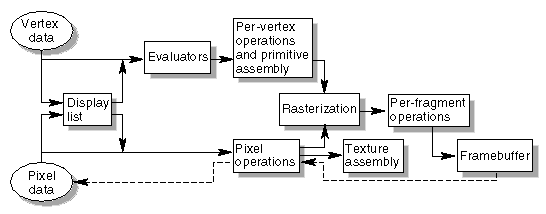
\includegraphics[width=0.9\linewidth]{images/chapter_stato_arte/stato_arte_opengl_pipeline.png}\hfill
 \caption[Pipeline di rendering di OpenGL]{Pipeline di rendering di OpenGL.}
 \label{fig:stato_arte_opengl_pipeline}
\end{figure}
\\
Tutti i dati, ad esempio delle descrizioni di geometrie, o delle descrizioni di pixel, vengono inizialmente memorizzati in una lista di elementi da renderizzare, detta \emph{display list}. Gia da questo punto è possibile istruire la pipeline affinchè, invece di memorizzare temporaneamente i dati in una lista, li processi immediatamente. 
\\
Una volta estratti i dati dalla lista inizia il processamento vero e proprio dei dati. La prima fase prevede che alla fine tutte le primitive geometriche siano descritte mediante vertici. Per ottenere ciò è necessario che tutte le primitive in input siano valutate in modo da individuare casi particolari come le curve parametriche, le quali sono descritte da punti di controllo e da funzioni polinomiali chiamate funzioni base. 
\\
In tal caso uno strumento di valutazione farà uso di un metodo di mappatura polinomiale per ottenere dai punti di controllo i vertici usati per rappresentare la superficie. Inoltre questo metodo consente di estrarre dai punti di controllo anche informazioni come normali di faccia, coordinate di texture e colore. 
\\
A questo punto le coordinate di ogni vertice vengono proiettate nel sistema di riferimento della camera mediante la matrice modello-vista. Inoltre, se abilitati, vengono calcolati gli effetti luminosi utilizzando i vertici proiettati, le normali  e le informazioni sul materiale e sulle luci; il risultato di questo calcolo sarà un colore.
\\
Il flusso di vertici viene interpretato in modo diverso a seconda di come è stata istruita la pipeline di rendering. Vi è infatti una informazione di connettività tra vertici che determina come i vertici devono essere connessi per creare una sequenza di primitive base. 
\\
Attraverso l’informazione di connettività dei vertici si può scegliere se le primitive base dovranno essere punti, linee, o poligoni. Ad esempio si supponga di avere una sequenza di sei vertici, e che l’informazione di connettività tra vertici indichi che il rendering deve utilizzare triangoli; l’interpretazione del flusso di sei vertici avrà come risultato due triangoli. 
L’output di questa fase è quindi composto da primitive geometriche base, insieme alle informazione sul colore, profondità, e altre informazioni utili alle fase di rasterizzazione.
\\
\begin{figure}[htb]
 \centering
 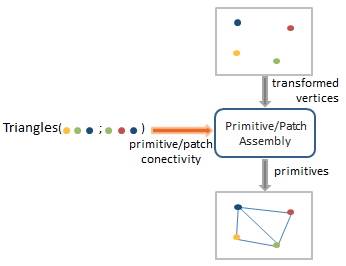
\includegraphics[width=0.5\linewidth]{images/chapter_stato_arte/stato_arte_prim_ass.png}\hfill
 \caption[Primitive Assembly]{Un'esempio di interpretazione delle primitive geometriche in base all'informazione di connettività fornita.}
 \label{fig:stato_arte_prim_ass}
\end{figure}
\\
Come visto nella prima fase della pipeline, la lista degli elementi da renderizzare può contenerei anche informazioni sui pixel, oltre che sulle geometrie. Mentre queste ultime sono soggette ai processamenti sopra descritti, i dati sui pixel vengono elaborati diversamente.
Per prima cosa i dati sono estratti dalla lista e copiati in una unità di memorizzazione governata da OpenGL in cui vige un determinato formato di immagine; di base esistono tre tipi di formato immagine:
\begin{itemize}
\item Colore: vengono memorizzati i colori in formato RGBA, ovvero ogni colore avrà una componente di rosso R, di verde G, e di blu B, e una componente alpha, usata solitamente dallo shader come valore di traslucenza, ma non solo. In generare viene sfruttata in modo diverso a seconda di come è stato istruito lo shader.
\item Profondità: questo formato memorizza le informazioni sulla profondità, necessarie  per i test di profondità sul depth buffer.
\item Profondità/Stencil: questo formato combina informazione di stencil e di profondità, e permette di allocare sia uno stencil buffer che un depth buffer.
\end{itemize}
La pipeline di rendering viene istruita in base al tipo di formato da adottare, influenzando così il modo in cui il dato deve essere interpretato.
Il trasferimento dei dati nella memoria di OpenGL è detto unpack.
Dopo lo spacchettamento dei dati, questi vengono scalati e processati mediante una mappa di pixel, e vengono ridimensionati in base al tipo di dato. Dopodichè vengono memorizzati in una area dedicata alle texture, per poi essere usati per la mappatura delle texture, o per essere dati in pasto al rasterizzatore. 
Per essere memorizzati in questa area, i dati sono prima raccolti in oggetti texture. Se nello stesso momento sono salvati troppi oggetti nella memoria texture, verranno mantenuti in memoria solo  gli oggetti texture ad alta priorità. 

A questo punto inizia il processo di rasterizzazione, in cui i dati sui pixel e quelli sulle geometrie, vengono convertiti in frammenti: partendo da una griglia di pixel in coordinate finestra, si individuano i pixel della griglia occupati dalle primitive. Successivamente ad ognuno di questi pixel si associa colore e profondità, ottenendo così un frammento. 
\\
\begin{figure}[htb]
 \centering
 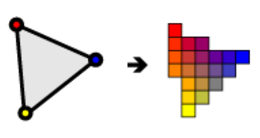
\includegraphics[width=0.4\linewidth]{images/chapter_stato_arte/stato_arte_raster.png}\hfill
 \caption[Rasterizzazione OpenGL]{Processo di rasterizzazione.}
 \label{fig:stato_arte_raster}
\end{figure}

Ogni frammento con coordinate di finestra $(x_w,y_w)$ prodotto dalla rasterizzazione, modificherà il pixel nel framebuffer che si trova nella stessa posizione in base a determinati parametri e condizioni. Questi sono valutati attraverso una serie di operazioni sui frammenti, mostrate in figura \ref{fig:stato_arte_frag_op}
\begin{figure}[htb]
 \centering
 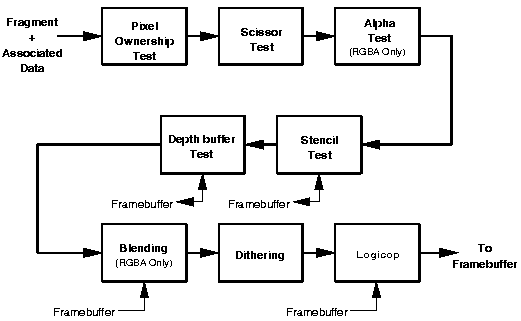
\includegraphics[width=0.9\linewidth]{images/chapter_stato_arte/stato_arte_frag_op.png}\hfill
 \caption[Operazioni sui frammenti]{Operazioni sui frammenti generati nella fase di rasterizzazione di OpenGL.}
 \label{fig:stato_arte_frag_op}
\end{figure}
\emph{Pixel ownership test} : si valuta se il pixel in posizione $(x_w,y_w)$ è presente nel framebuffer. Se non è presente, il frammento potrebbe essere scartato, oppure processato solamente da un sottoinsieme delle operazioni sui frammenti.
\\

\emph{Scissor test} : vengono scartati i frammenti al di fuori di una certa porzione rettangolare dello schermo definita mediante una funzione; questo test si può attivare o meno mediante \texttt{glEnable()} o \texttt{glDisable()} sulla variabile corrispondente allo stato di questo test. Se disattivato, il test avrà sempre esito positivo.
\\

\emph{Alpha test} : viene confrontato il valore alpha del frammento, con un valore di riferimento; il tipo di confronto $(>,\geq,<,\leq)$ dipende dalla costante scelta tra quelle offerte da OpenGL: never, always, equal, gequal, lequal, ecc.
\\

\emph{Stencil test} : viene confrontato i valore dello stencil buffer nella posizione $(x_w,y_w)$ del frammento con un valore di riferimento. Se il test ha esito negativo, il frammento viene scartato.
\\

\emph{Depth buffer test} : viene confrontato il valore del depth buffer nella posizione $(x_w,y_w)$ del frammento, con il valore $z_w$ del frammento stesso. Se il test non da esito positivo, il frammento viene scartato.
\\

\emph{Blending} : data la posizione $(x_w,y_w)$ del frammento, e la sua componente di colore RGBA, si prende la componente RGBA del pixel in posizione $(x_w,y_w)$ nel framebuffer, e la si combina con quella del frammento.
\\

\emph{Dithering} : Prima di spiegare questo processo è necessaria una premessa, ossia che per ogni pixel vengono memorizzate delle informazioni sui colori, e la quantità di informazioni memorizzata dipende dal numero di bitplanes che il sistema alloca al framebuffer.
Ad esempio se avessimo un 1 bitplane per l’informazione di colore di un pixel, per ogni pixel potremmo memorizzare l’informazione di colore in 1 bit; con 8 bitplanes avremmo 8 bit di informazione, e quindi 256 tonalità di colore possibili da memorizzare. 
\\
Ovviamente la quantità di bitplanes che un sistema alloca al framebuffer non può essere infinita, pertanto se si vuole aumentare la quantità di colori rappresentabili bisogna ricorre ad uno stratagemma; questo stratagemma è detto dithering, e a grandi linee il funzionamento è il seguente: supponiamo che la quantità di bitplanes allocata per le informazioni di colore non sia sufficiente a memorizzare il rosa, e supponiamo che un poligono necessiti questa colorazione. 
\\
Il dithering agisce in questo caso creando per l’occhio umano un illusione ottica, facendo apparire il poligono rosa quando in verità non lo è. Questa illusione è possibile coprendo l’area del poligono con un motivo “a scacchi”, dove ogni casella, ossia un pixel, assumerà una colorazione tra quelle disponibili nelle informazioni di colore, con l’obiettivo di ottenere come risultato complessivo, una tonalità di colore mancante nelle informazioni dei pixel. Ad esempio l’illusione del rosa è ottenibile alternando, in un motivo a scacchi, pixel rossi con pixel bianchi. Un tecnica simile al dithering è usata per rappresentare scale di grigi nelle foto dei quotidiani in bianco e nero.
\\

\emph{Logical operation}: L’ultimo passo corrisponde ad una serie di operazioni logiche tra colore e posizione del frammento, e colore e posizione del pixel nel framebuffer associato al frammento. Il risultati sostituiranno i valori del framebuffer nella posizione $(x_w,y_w)$ del frammento.
\\

Alcune implementazioni di OpenGL sono in grado di funzionare anche se il computer attraverso cui l’utente osserva il render di una scena è diverso dal computer che l’ha renderizzata.
Questa situazione è possibile se i computer sono connessi tra di loro mediante infrastruttura di rete.
\\
In un ambiente di questo tipo la macchina sulla quale è installato il software grafico, il quale traduce i comandi dell’utente in chiamate a funzioni di OpenGL, è detto client; questa è la macchina con cui l’utente sta interagendo. 
\\
La macchina che riceve le chiamate a funzione di OpenGL, e che processa la pipeline di render, è detta server. Il formato di interscambio di informazioni tra client e server è sempre lo stesso; in questo modo il programma OpenGL può funzionare in ambiente distribuito anche se le macchine comunicanti sono di diverso tipo. Se invece non è previsto che la specifica implementazione di OpenGL operi attraverso la rete, allora avremo un solo calcolatore che fungerà sia da client che da server.
